\documentclass[answers]{exam}
\usepackage[english]{babel}
\usepackage[utf8x]{inputenc}
\usepackage{amsmath,amssymb,amsthm,mathtools}

\title{OPER 510 - Introduction to Mathematical Programming%
	\\ Midterm}
\author{Brandon Hosley}
\date{\today}

\usepackage[table,dvipsnames]{xcolor}
\usepackage{graphicx}
\usepackage{nicefrac}
\usepackage{enumitem}
\usepackage{multicol}
\usepackage{setspace}
\usepackage[final]{pdfpages}

\begin{document}
\includepdf[pages=-]{Midterm Agreement Signed.pdf}
\maketitle
\unframedsolutions

\begin{questions}
	
%%%%%%%%%%%%%%%%%%%%%%%%%%%
% 	\begin{ Question 1}	  %
%%%%%%%%%%%%%%%%%%%%%%%%%%%
\question
\begin{parts}
	\part Via the simplex method, find the solution to the following problem:
	\begin{flalign*}
		\text{Max } z=90x_1 +40x_2 +10x_3 +30x_4            &         &  \\
		\text{s.t.}\hspace{2.5em} 15x_1 +10x_2 +10x_3 + \,\ 5x_4 & \leq 45 &  \\
		15x_1+ \,\ 5x_2+ \,\ 5x_3+ \,\ 5x_4                             & \leq 35 &  \\
		x_1 \hspace{22.5ex}                                    & \geq 1  &  \\
		x_3 \hspace{7ex}                                    & \geq 2  &  \\
		x_1,x_2,x_3,x_4                                     & \geq 0  &
	\end{flalign*}

	\part The General Service Organization, GSO, has contracted to sell certain quantities of a particular product over the next four months. Because of variations in the size of the labor force, the production capacity and materials, costs vary from month to month. Storage costs are incurred on any items carried over to the next month, but not on items sold in the same month that they are produced. The costs and requirements are summarized below: \bigskip \\
	\begin{tabular}{ccccc}
		& Contracted & Production & Production & Storage \\
		\underline{Month} & \underline{Sales} & \underline{Capacity} & \underline{Cost/Unit (\$)} & \underline{Cost/Unit/Month (\$)} \\
		1 & 60 & 90 & 70 & 2 \\
		2 & 70 & 60 & 72 & 1 \\
		3 & 90 & 80 & 70 & 1 \\
		4 & 70 & 100 & 65 & 3 \\
	\end{tabular} \bigskip \\
	Initial inventory is 20 units. For service reasons, GSO wants to maintain at least 5 units of inventory at the end of each month. \textit{Formulate} a linear programming model to determine GSO’s production and inventory schedule.
	
	\part Give the rank of the following system of equations: 
	\begin{flalign*}
		2x_1 +\ \ 3x_2 +4x_3 &=3 &\\
		4x_1 +\ \ 5x_2 +1x_3 &=2 &\\
		 x_1 +1.5x_2 +2x_3 &=3/2 &\\
	\end{flalign*}
	
	\part Solve the following linear program.
	\begin{flalign*}
		\text{Max } z=10x_1 +3x_2 +12x_3 & & \\
		\text{s.t.}\hspace{3em} 2x_1 +1x_2+ \,\ 5x_3 &\leq 20 & \\
		x_1, x_2, x_3 &\geq 0 & \\
	\end{flalign*}
\end{parts}

\begin{solution}
\begin{parts}
	\part % Q1-A
	\noindent \\
	\begin{tabular}{cccccccccccccc}
		$c_j$                   &                            &                                & 90    & 40    & 10    & 30    & 0     & 0     & 0     & 0     & -M    & -M    &           \\
		\multicolumn{1}{c|}{}   & \multicolumn{1}{c|}{bv}    & \multicolumn{1}{c|}{RHS}       & $x_1$ & $x_2$ & $x_3$ & $x_4$ & $s_1$ & $s_2$ & $s_3$ & $s_4$ & $A_1$ & $A_2$ & ratio     \\ \cline{1-13}
		\multicolumn{1}{c|}{0}  & \multicolumn{1}{c|}{$s_1$} & \multicolumn{1}{c|}{45}        & 15    & 10    & 10    & 5     & 1     & 0     & 0     & 0     & 0     & 0     & 45/15=3   \\
		\multicolumn{1}{c|}{0}  & \multicolumn{1}{c|}{$s_2$} & \multicolumn{1}{c|}{35}        & 15    & 5     & 5     & 5     & 0     & 1     & 0     & 0     & 0     & 0     & 35/15=2.3 \\
		\multicolumn{1}{c|}{-M} & \multicolumn{1}{c|}{$A_1$} & \multicolumn{1}{c|}{1}         & 1     & 0     & 0     & 0     & 0     & 0     & -1    & 0     & 1     & 0     & 1/1=1     \\
		\multicolumn{1}{c|}{-M} & \multicolumn{1}{c|}{$A_2$} & \multicolumn{1}{c|}{2}         & 0     & 0     & 1     & 0     & 0     & 0     & 0     & -1    & 0     & 1     & 0         \\ \cline{1-13}
		& \multicolumn{1}{c|}{$z_j$} & \multicolumn{1}{c|}{-2M}       & -M    & 0     & -M    & 0     & 0     & 0     & M     & M     & -M    & -M    &           \\ \cline{3-13}
		&                            & \multicolumn{1}{c|}{$c_j-z_j$} & 90+M  & 0     & 10+M  & 0     & 0     & 0     & -M    & -M    & 0     & 0     &          
	\end{tabular} \\
	Enter on $x_1$, exit $A_1$ \\
	R1 - 15R3 \\
	R2 - 15R3 \\
	\begin{tabular}{cccccccccccccc}
		$c_j$                   &                            &                                & 90    & 40    & 10    & 30    & 0     & 0     & 0     & 0     & -M    & -M    &         \\
		\multicolumn{1}{c|}{}   & \multicolumn{1}{c|}{bv}    & \multicolumn{1}{c|}{RHS}       & $x_1$ & $x_2$ & $x_3$ & $x_4$ & $s_1$ & $s_2$ & $s_3$ & $s_4$ & $A_1$ & $A_2$ & ratio   \\ \cline{1-13}
		\multicolumn{1}{c|}{0}  & \multicolumn{1}{c|}{$s_1$} & \multicolumn{1}{c|}{30}        & 0     & 10    & 10    & 5     & 1     & 0     & 15    & 0     & 0     & 0     & 30/10=3 \\
		\multicolumn{1}{c|}{0}  & \multicolumn{1}{c|}{$s_2$} & \multicolumn{1}{c|}{20}        & 0     & 5     & 5     & 5     & 0     & 1     & 15    & 0     & 0     & 0     & 20/5=4  \\
		\multicolumn{1}{c|}{90} & \multicolumn{1}{c|}{$x_1$} & \multicolumn{1}{c|}{1}         & 1     & 0     & 0     & 0     & 0     & 0     & -1    & 0     & 1     & 0     & 0       \\
		\multicolumn{1}{c|}{-M} & \multicolumn{1}{c|}{$A_2$} & \multicolumn{1}{c|}{2}         & 0     & 0     & 1     & 0     & 0     & 0     & 0     & -1    & 0     & 1     & 2/1=2   \\ \cline{1-13}
		& \multicolumn{1}{c|}{$z_j$} & \multicolumn{1}{c|}{90-2M}     & 90    & 0     & -M    & 0     & 0     & 0     & -90   & M     & 90    & -M    &         \\ \cline{3-13}
		&                            & \multicolumn{1}{c|}{$c_j-z_j$} & 0     & 40    & 10+M  & 0     & 0     & 0     & 90    & -M    & -M-90 & 0     &        
	\end{tabular} \\
	Enter $x_3$, exit $A_2$ \\
	R1 - 10R4 \\
	R2 - 5R4 \\
	\begin{tabular}{cccccccccccccc}
		$c_j$                   &                            &                                & 90    & 40    & 10    & 30    & 0     & 0     & 0     & 0     & -M    & -M    &           \\
		\multicolumn{1}{c|}{}   & \multicolumn{1}{c|}{bv}    & \multicolumn{1}{c|}{RHS}       & $x_1$ & $x_2$ & $x_3$ & $x_4$ & $s_1$ & $s_2$ & $s_3$ & $s_4$ & $A_1$ & $A_2$ & ratio     \\ \cline{1-13}
		\multicolumn{1}{c|}{0}  & \multicolumn{1}{c|}{$s_1$} & \multicolumn{1}{c|}{10}        & 0     & 10    & 0     & 5     & 1     & 0     & 15    & 10    & -15   & -10   & 10/15=0.6 \\
		\multicolumn{1}{c|}{0}  & \multicolumn{1}{c|}{$s_2$} & \multicolumn{1}{c|}{10}        & 0     & 5     & 0     & 5     & 0     & 1     & 15    & 5     & 0     & -5    & 10/15=0.6 \\
		\multicolumn{1}{c|}{90} & \multicolumn{1}{c|}{$x_1$} & \multicolumn{1}{c|}{1}         & 1     & 0     & 0     & 0     & 0     & 0     & -1    & 0     & 1     & 0     & 1/-1=-1   \\
		\multicolumn{1}{c|}{10} & \multicolumn{1}{c|}{$x_3$} & \multicolumn{1}{c|}{2}         & 0     & 0     & 1     & 0     & 0     & 0     & 0     & -1    & 0     & 1     & 0         \\ \cline{1-13}
		& \multicolumn{1}{c|}{$z_j$} & \multicolumn{1}{c|}{110}       & 90    & 0     & 10    & 0     & 0     & 0     & -90   & -10   & 90    & 10    &           \\ \cline{3-13}
		&                            & \multicolumn{1}{c|}{$c_j-z_j$} & 0     & 40    & 0     & 30    & 0     & 0     & 90    & 10    & -M-90 & -M-10 &          
	\end{tabular} \\
	Enter $s_3$, exit $s_2$ \\
	R2 / 15 \\
	R1 - 15R2 \\
	R3 + R2 \\
	\begin{tabular}{cccccccccccccc}
		$c_j$                   &                            &                                & 90    & 40    & 10    & 30    & 0     & 0     & 0     & 0     & -M    & -M    &               \\
		\multicolumn{1}{c|}{}   & \multicolumn{1}{c|}{bv}    & \multicolumn{1}{c|}{RHS}       & $x_1$ & $x_2$ & $x_3$ & $x_4$ & $s_1$ & $s_2$ & $s_3$ & $s_4$ & $A_1$ & $A_2$ & ratio         \\ \cline{1-13}
		\multicolumn{1}{c|}{0}  & \multicolumn{1}{c|}{$s_1$} & \multicolumn{1}{c|}{0}         & 0     & 5     & 0     & 0     & 1     & -1    & 0     & 5     & -15   & -5    &               \\
		\multicolumn{1}{c|}{0}  & \multicolumn{1}{c|}{$s_3$} & \multicolumn{1}{c|}{2/3}       & 0     & 1/3   & 0     & 1/3   & 0     & 1/15  & 1     & 1/3   & 0     & -1/3  & (2/3)/(1/3)=2 \\
		\multicolumn{1}{c|}{90} & \multicolumn{1}{c|}{$x_1$} & \multicolumn{1}{c|}{5/3}       & 1     & 1/3   & 0     & 1/3   & 0     & 1/15  & 0     & 1/3   & 1     & -1/3  & (5/3)/(1/3)=5 \\
		\multicolumn{1}{c|}{10} & \multicolumn{1}{c|}{$x_3$} & \multicolumn{1}{c|}{2}         & 0     & 0     & 1     & 0     & 0     & 0     & 0     & -1    & 0     & 1     &               \\ \cline{1-13}
		& \multicolumn{1}{c|}{$z_j$} & \multicolumn{1}{c|}{170}       & 90    & 30    & 10    & 30    & 0     & 6     & 0     & 20    & 90    & -20   &               \\ \cline{3-13}
		&                            & \multicolumn{1}{c|}{$c_j-z_j$} & 0     & 10    & 0     & 0     & 0     & -6    & 0     & -20   & 90-M  & -20-M &              
	\end{tabular} \\
	Enter $x_2$ exit $s_3$ \\
	R2 x 3 \\
	R1 - 5R2 \\
	R3 - 1/3R2 \\
	\begin{tabular}{cccccccccccccc}
		$c_j$                   &                            &                                & 90    & 40    & 10    & 30    & 0     & 0     & 0     & 0     & -M    & -M    &       \\
		\multicolumn{1}{c|}{}   & \multicolumn{1}{c|}{bv}    & \multicolumn{1}{c|}{RHS}       & $x_1$ & $x_2$ & $x_3$ & $x_4$ & $s_1$ & $s_2$ & $s_3$ & $s_4$ & $A_1$ & $A_2$ & ratio \\ \cline{1-13}
		\multicolumn{1}{c|}{0}  & \multicolumn{1}{c|}{$s_1$} & \multicolumn{1}{c|}{-10}       & 0     & 0     & 0     & -5    & 1     & -2    & 0     & 0     & -15   & -10   &       \\
		\multicolumn{1}{c|}{40} & \multicolumn{1}{c|}{$x_2$} & \multicolumn{1}{c|}{2}         & 0     & 1     & 0     & 1     & 0     & 1/5   & 3     & 1     & 0     & -1    &       \\
		\multicolumn{1}{c|}{90} & \multicolumn{1}{c|}{$x_1$} & \multicolumn{1}{c|}{1}         & 1     & 0     & 0     & 0     & 0     & 0     & -1    & 0     & 1     & 0     &       \\
		\multicolumn{1}{c|}{10} & \multicolumn{1}{c|}{$x_3$} & \multicolumn{1}{c|}{2}         & 0     & 0     & 1     & 0     & 0     & 0     & 0     & -1    & 0     & 1     &       \\ \cline{1-13}
		& \multicolumn{1}{c|}{$z_j$} & \multicolumn{1}{c|}{190}       & 90    & 40    & 30    & 40    & 0     & 8     & 30    & 30    & 90    & -30   &       \\ \cline{3-13}
		&                            & \multicolumn{1}{c|}{$c_j-z_j$} & 0     & 0     & 0     & -10   & 0     & -8    & -30   & -30   & 90-M  & -30-M &      
	\end{tabular} \\

	\textbf{Summary: } The optimal values will be $x_1=1, x_2=2, x_3=2, x_4=0$ for a maximum $z=190$.
	
	\part % Q1-B 
	The situation described may look like this chart. \\
	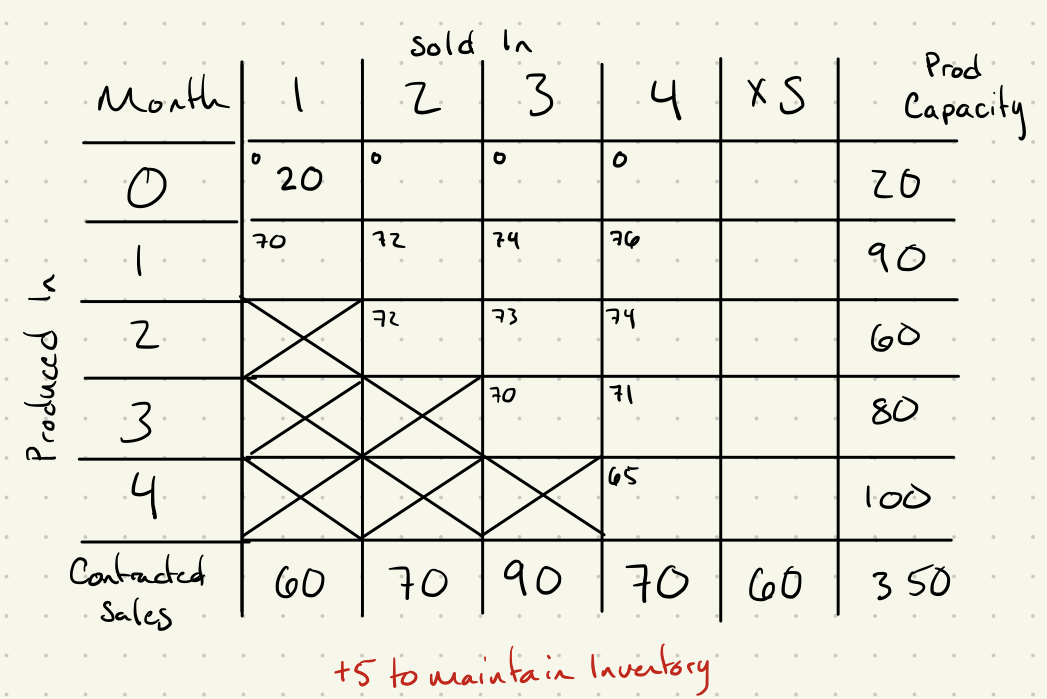
\includegraphics[width=.5\linewidth]{TransportGraph} \\
	The system of linear equations representing this situation 
	will be presented below and will use the following variables: \\
	$z:$ Production costs, \\
	$x_{ps}:$ Products produced in month $p$ and sold in month $s$, \\
	$x_0:$ Is the initial inventory, \\
	$s_p:$ Slack in production capacity for month $p$. \\
	\textbf{Linear System Formulated: }
	\begin{flalign*}
		&\text{Min } z = 70x_{11} + 72x_{12} + 74x_{13} + 76x_{14} +72x_{22} + 73x_{23} + 74x_{24} + 70x_{33} + 71x_{34} + 65x_{44}  & \\
		&\text{s.t.}  & 
	\end{flalign*} \vspace{-3em} % x_{} 
	\begin{flalign*}
		\intertext{Contracted Sales + GSO Inventory Constraints}
		x_0 + x_{11} \hspace{18ex} &\geq 65 & \\
		x_0 + x_{12} + x_{22} \hspace{12ex} &\geq 75 & \\
		x_0 + x_{13} + x_{23} + x_{33} \hspace{6ex} &\geq 95 & \\
		x_0 + x_{14} + x_{24} + x_{34} + x_{44} &\geq 75 & \\
		\intertext{Production Capacity Constraints}
		x_0 + s_0 &= 20 & \\
		x_{11} + x_{12} + x_{13} + x_{14} + s_1 &= 90 & \\
		x_{22} + x_{23} + x_{24} + s_2 &= 60 & \\
		x_{33} + x_{34} + s_3 &= 80 & \\
		x_{44} + s_4 &= 100 & 
		\intertext{Physics Constraints}
		x_{11}, x_{12}, x_{13}, x_{14}, x_{22}, x_{23}, x_{24},x_{33}, x_{34}, x_{44}, s_1, s_2, s_3, s_4 &\geq 0 \\
		x_{21}, x_{31}, x_{32}, x_{41}, x_{42}, x_{43} &= 0
	\end{flalign*}
	
	\part % Q1-C
	\begin{align*} % \xRightarrow[below]{above}
		&\begin{bmatrix}
			2 & 3 & 4 & 3 \\
			4 & 5 & 1 & 2 \\
			1 & 1.5 & 2 & 3/2 \\
		\end{bmatrix}
		\xRightarrow[R1=R1/2]{R3=R3-2R1}
		\begin{bmatrix}
			1 & 1.5 & 2 & 1.5 \\
			4 & 5 & 1 & 2 \\
			0 & 0 & 0 & 0 \\
		\end{bmatrix} 
		\xRightarrow[R1=R1+1.5R2]{R2=R2-4R1} \\
		&\begin{bmatrix}
			1 & 0 & -8.5 & -4.5 \\
			0 & -1 & -7 & -4 \\
			0 & 0 & 0 & 0 \\
		\end{bmatrix}
	\xRightarrow[]{R2=-R2}
	\begin{bmatrix}
		1 & 0 & -8.5 & -4.5 \\
		0 & 1 & 7 & 4 \\
		0 & 0 & 0 & 0 \\
	\end{bmatrix}
	\end{align*}
	
	\textbf{Summary: } The rank of the provided system of equations is 2. As a result, $x_3$ is a free-variable, and there are infinitely many solutions.
	
	\part % Q1-D
	Contribution to $z$: $x_1 = 10/2, x_2=3/1, x_3=12/5$ \\
	Since $x_1$ is the largest, we will maximize it.
	
	\textbf{Summary: } The optimal arrangement will be 
	$x_1=10, x_2=0, x_3=0$ for a maximum $z=100$.
	
\end{parts}
\end{solution}
%\end{ Question 1}

%%%%%%%%%%%%%%%%%%%%%%%%%%%
% 	\begin{ Question 2}	  %
%%%%%%%%%%%%%%%%%%%%%%%%%%%
\question
\begin{parts}
	\part Show that for $a \geq$ constraint $i$ in a maximization problem 
	that $y_i = −(\bar{c}_{BV} B^{−1}\bar{a}_{n+i} )$ 
	
	\part State the dual of the following linear program.
	\begin{flalign*}
		\text{Min } z=3x_1 +7x_2 −15x_3 +43x_4 & & \\
		\text{s.t.} \hspace{2.5em} 
		10x_1 +6x_2 +4x_3 +13x_4 &\leq 100 & \\
		−2x_1 + 3x_2 −5x_3 \hspace{7ex}\, &\geq 200 & \\
		12x_1 −3x_2 +2x_3 +22x_4 &\geq 225 & \\
		x_1,x_3,x_4 \geq 0 x_2 \text{urs} & & \\ 
	\end{flalign*}
	
	\part Given the following final tableau for a maximization problem with all less than or equal to constraints, state the original model. \\
	\begin{tabular}{lllllllll}
		$z$ & $x_1$ & $x_2$ & $x_3$ & $x_4$ & $x_5$ & RHS & BV    & Ratio \\ \hline
		1   & 0     & 0     & 0     & 3/2   & 1     & 36  & Z     &       \\
		0   & 0     & 0     & 1     & 1/3   & -1/3  & 2   & $x_3$ &       \\
		0   & 0     & 1     & 0     & 1/2   & 0     & 6   & $x_2$ &       \\
		0   & 1     & 0     & 0     & -1/3  & 1/3   & 2   & $x_1$ &      
	\end{tabular}
	
\end{parts}

\begin{solution}
	\begin{parts}
		\part % Q2-A
		
		
		\part % Q2-B
		\textbf{Summary: } The dual of the provided system is:
		\begin{flalign*}
			\text{Max } z = -100y_1 +200y_2 +225y_3 & & \\
			\text{s.t. }\hspace{2.5em}
			-10y_1 -\quad\, 2y_2 +\ 12y_3 &\leq 3 & \\
			-6y_1 +\quad\ 3y_2 -\ \ 3y_3 &\leq 7 & \\
			-4y_1 -\quad\ 5y_2 +\ \ 2y_3 &\leq -15 & \\
			-13y_1 +\quad \qquad + \ 22y_3 &\leq 43 &
		\end{flalign*}
		
		\part % Q2-C
		\noindent \\
		Exit $x_1$, Re-add $x_5$ \\
		R3 x 3 \\
		R1 + 1/3R3 \\
		R0 - R3 \\
		\begin{tabular}{lllllllll}
			$z$ & $x_1$ & $x_2$ & $x_3$ & $x_4$ & $x_5$ & RHS & BV    & Ratio \\ \hline
			1   & -3    & 0     & 0     & 5/2   & 0     & 30  & Z     &       \\
			0   & 1     & 0     & 1     & 0     & 0     & 4   & $x_3$ &       \\
			0   & 0     & 1     & 0     & 1/2   & 0     & 6   & $x_2$ &       \\
			0   & 3     & 0     & 0     & -1    & 1     & 6   & $x_5$ &      
		\end{tabular} \\
		Exit $x_2$, through $x_4$ \\
		R2 x 2 \\
		R3 + R2 \\
		R0 - 5/2R2 \\
		\begin{tabular}{lllllllll}
			$z$ & $x_1$ & $x_2$ & $x_3$ & $x_4$ & $x_5$ & RHS & BV    & Ratio \\ \hline
			1   & -3    & -5    & 0     & 0     & 0     & 0   & Z     &       \\
			0   & 1     & 0     & 1     & 0     & 0     & 4   & $x_3$ &       \\
			0   & 0     & 2     & 0     & 1     & 0     & 12  & $x_4$ &       \\
			0   & 3     & 2     & 0     & 0     & 1     & 18  & $x_5$ &      
		\end{tabular} \bigskip \\
		\textbf{Summary: } The original model was such that the least common multiple of the coefficients would have have appeared as follows:
		\begin{flalign*}
			\text{Max } z = 3x_1 + 5x_2 & & \\
			\text{s.t.}\hspace{3em}
			x_1 \hspace{6ex} \, &\leq 4 & \\
			2x_2 & \leq 12 & \\
			3x_1 + 2x_2 & \leq 18 & \\
		\end{flalign*}
	\end{parts}
\end{solution}
%\end{ Question 2}

%%%%%%%%%%%%%%%%%%%%%%%%%%%
% 	\begin{ Question 3}	  %
%%%%%%%%%%%%%%%%%%%%%%%%%%%
\question
\begin{parts}
	\part % Q3-A
	\part % Q3-B
	\part % Q3-C
	\part % Q3-D
	\part % Q3-E
	\part % Q3-F
	\part % Q3-G
\end{parts}

\begin{solution}
	\begin{parts}
		\part % Q3-A
		\part % Q3-B
		\part % Q3-C
		\part % Q3-D
		\part % Q3-E
		\part % Q3-F
		\part % Q3-G
	\end{parts}
\end{solution}
%\end{ Question 3}

%%%%%%%%%%%%%%%%%%%%%%%%%%%
% 	\begin{ Question 4}	  %
%%%%%%%%%%%%%%%%%%%%%%%%%%%
\question
\begin{parts}
	\part Solve the following linear program:
	\begin{flalign*}
		\text{Min } z=4x_1 +5x_2 & & \\
		\text{s.t.} \hspace{2.5em} 
		3x_1 +1x_2 &\leq 27 & \\
		5x_1 +5x_2 &= 60 & \\
		6x_1 +4x_2 &\geq 60 & \\
		x1,x2 &\geq0 & 
	\end{flalign*}

	\part Consider the problem,
	\begin{flalign*}
		\text{Max } z =5x_1 +2x_2 +3x_3 & & \\
		\text{s.t.} \hspace{3em} 
		x_1 +5x_2 +2x_3 &\leq b_1 & \\
		x_1 −5x_2 −6x_3 &\leq b_2 & \\
		x_1,x_2,x_3 &\geq 0 & 
	\end{flalign*}
	where \(b_1\) and \(b_2\) are constants. For specific values of \(b1\) and \(b_2\), the optimal tableau is \\
	\begin{tabular}{ccccccc}
		$z$ & $x_1$ & $x_2$ & $x_3$ & $s_1$ & $s_2$ & RHS \\ \hline
		1   & 0     & $a$   & 7     & $d$   & $e$   & 150 \\
		0   & 1     & $b$   & 2     & 1     & 0     & 30  \\
		0   & 0     & $c$   & -8    & -1    & 1     & 10 
	\end{tabular} \\
	where \(a\), \(b\), \(c\), \(d\), and \(e\) are constants. Determine:
	\begin{subparts}
		\subpart The values of \(b_1\) and \(b_2\) that yield the given optimal solution.
		\subpart The values of \(a\), \(b\), and \(c\) in the optimal tableau.
	\end{subparts}
\end{parts}

\begin{solution}
	\begin{parts}
		\part % Q4-A
		\noindent \\
		\begin{tabular}{cccccccc}
			$z$ & $x_1$ & $x_2$ & $s_1$ & $s_2$ & $A_1$ & RHS & BV    \\ \hline
			1   & -4    & -5    & 0     & 0     & 0     & 0   & -z    \\
			0   & 3     & 1     & 1     & 0     & 0     & 27  & $s_1$ \\
			0   & 5     & 5     & 0     & 0     & 1     & 60  & $A_1$ \\
			0   & -6    & -4    & 0     & 1     & 0     & -60 & $s_2$
		\end{tabular}
		Leaving $A_1$, enter $x_1$ \\
		R3/5 \\
		R1 + 4R3 \\
		R2 - 3R3 \\
		R4 + 6R3 \\
		\begin{tabular}{cccccccc}
			$z$ & $x_1$ & $x_2$ & $s_1$ & $s_2$ & $A_1$ & RHS & BV    \\ \hline
			1   & 0     & -1    & 0     & 0     & 4/5   & 48  & -z    \\
			0   & 0     & -2    & 1     & 0     & -3/5  & -9  & $s_1$ \\
			0   & 1     & 1     & 0     & 0     & 1/5   & 12  & $x_1$ \\
			0   & 0     & 2     & 0     & 1     & 6/5   & 12  & $s_2$
		\end{tabular} \\
		Leaving $s_1$, enter $x_2$ \\
		R2/-2 \\
		R1 + R2 \\
		R3 - R2 \\
		R4 - 2R2 \\
		\begin{tabular}{cccccccc}
			$z$ & $x_1$ & $x_2$ & $s_1$ & $s_2$ & $A_1$ & RHS  & BV    \\ \hline
			1   & 0     & 0     & -1/2  & 0     & 11/10 & 52.5 & -z    \\
			0   & 0     & 1     & -1/2  & 0     & 3/10  & 4.5  & $x_2$ \\
			0   & 1     & 0     & 1/2   & 0     & -1/10 & 7.5  & $x_1$ \\
			0   & 0     & 0     & 1     & 1     & 6/10  & 3    & $s_2$
		\end{tabular} \bigskip \\
		\textbf{Summary: } The optimal situation is $x_1=7.5$ and $x_2=4.5$ for a minimum $z=52.5$.
		
		\part % Q4-B
		\begin{subparts}
			\subpart % Q4-B-1
			The known values in R2 match the values in the original constraints,
			and since $x_1$ has no coefficient, $b_1=30$. 
			Simple substitution into the second constraint or by adding the slack in R3
			gives $b_2=40$.
			\subpart % Q4-B-2
			As above, the values of R2 are unchanged, so $b=5$. 
			Then, undoing the changes to the other rows reveals the remaining numbers.
			For R3, subtracting R2 from the original constraint gives the final R3 and $c=-10$.
			For R1, adding 5R2 to the original function matches the knowns and gives $a=23$.
		\end{subparts}
	\end{parts}
\end{solution}
%\end{ Question 4}

%%%%%%%%%%%%%%%%%%%%%%%%%%%
% 	\begin{ Question 5}	  %
%%%%%%%%%%%%%%%%%%%%%%%%%%%
\question
\begin{parts}
	\part % 5-A
	Consider the following model:
	\begin{flalign*}
		\text{Max} z=3x_1 +1x_2 +2x_3 & & \\
		\text{s.t.} \hspace{2.5em}
		1x_1 −1x_2 +2x_3 &\leq20 & \\
		2x_1 +1x_2 −3x_3 &\leq10 & \\
		x_1,x_2,x_3 &\geq 0 & \\
	\end{flalign*}
	The Final tableau for this problem is: \\
	\begin{tabular}{cccccccc}
		$z$ & $x_1$ & $x_2$ & $x_3$ & $x_4$ & $x_5$ & RHS & BV    \\ \hline
		1   & 8     & 0     & 0     & 3     & 4     & 100 & $z$   \\
		0   & 3     & 0     & 1     & 1     & 1     & 30  & $x_3$ \\
		0   & 5     & 1     & 0     & 1     & 2     & 40  & $x_2$
	\end{tabular} \bigskip \\
	Consider each question below separately; i.e. without regard to the previous question.
	\begin{subparts}
		\subpart % 5-A-i
		Give the range for 1) $b_1$ and 2) $b_2$ over which each could individually range, all other items constant, and maintain the same optimal basis.
		\subpart % 5-A-ii
		If the profit on $c_2$ increased to 5, would the current basis remain optimal?
		\subpart % 5-A-iii
		The organization for which the above model was solved is considering adding a new product, $x_N$. This product uses 2 units of resource 1 and 5 units of resource 2. It’s contribution to profits is \$20 per unit. Should this product be produced? If it is produced, how much should be made?
	\end{subparts}
	\part % 5-B 
	Solve the following goal programming model via the \textbf{simplex method} for goal programs.
	Clearly identify the solution and the level of goal achievement.
	\begin{flalign*}
		\text{Min } z = P_1p_3 + P_2n_4 + P_2p_4 \hspace{20ex}& & \\
		\text{s.t.} \hspace{2.5em} 
		10x_1 +20x_2 +n_1 \hspace{22ex} & =1000 & \\
		20x_1 +10x_2 \hspace{4ex} +n_2 \hspace{18ex} &=800 & \\ 
		5x_1 +10x_2 \hspace{9ex} + n_3 - p_3 \hspace{8ex} &=600 & \\ 
		x_2 \hspace{17ex} + n_4 - p_4 &= 30 &\\
		x_1,x_2,n_1,n_2, n_3,p_3,n_4,p_4 &\geq 0 &
	\end{flalign*}
\end{parts}

\begin{solution}
	\begin{parts}
		\part % 5-A
		\begin{subparts}
			\subpart % 5-A-i
			\subpart % 5-A-ii
			\subpart % 5-A-iii
		\end{subparts}
		\part % 5-B
	\end{parts}
\end{solution}
%\end{ Question 5}

\end{questions}
\end{document}